\chapter{Assessment}\label{chp:assessment}

\section{Introduction}

This chapter will discuss the implementations in the previous chapter. Intended functionality and performance is compared to the actual results, and usefulness in the context of autonomous navigation is assessed. The assessments will be mostly qualitative.

\section{Vanishing Point Detection}

The vanishing point detector failed work as intended. Both the \gls{dsam} algorithm and the vanishing point detector itself is unable to fulfil their intended tasks. 

\subsection{What is Working?}

The application is stable and responsive as long as the \gls{dsam} algorithm is left out. While eliminating all errors and bugs was too time consuming to be completed, testing showed that the vanishing point voting scheme is working. It could be that the error is caused by mixing two coordinate systems. 

\subsection{Suitability for Autonomous navigation}

There are examples of robots that can successfully track  vanishing points\cite{monocularvp}, and even more examples where lines and edges are used in road detection and lane keeping. Methods based on perspective lines seems to be better suited for highly structured environments like roads, corridors and hallways than navigation in potentially cluttered areas.

\section{Depth Perception and Obstruction Detection}

\subsection{Stereo Matching}

\paragraph{Weaknesses}

The stereo matching process has two significant weaknesses: inability to detect texture-less surfaces, and false disparities from repetitive patterns. It may be that the matching parameters can be tuned in order to achieve denser disparity maps. On the other hand, the input images from the IP cameras are quite noisy, which makes the matching process much more difficult. It is possible that certain areas of the images, where the distinctive features are faint, are especially sensitive to noise. This results in a sparse disparity map, which can be unsuitable in applications such as 3d reconstruction and mapping of the environment.

\begin{figure}
	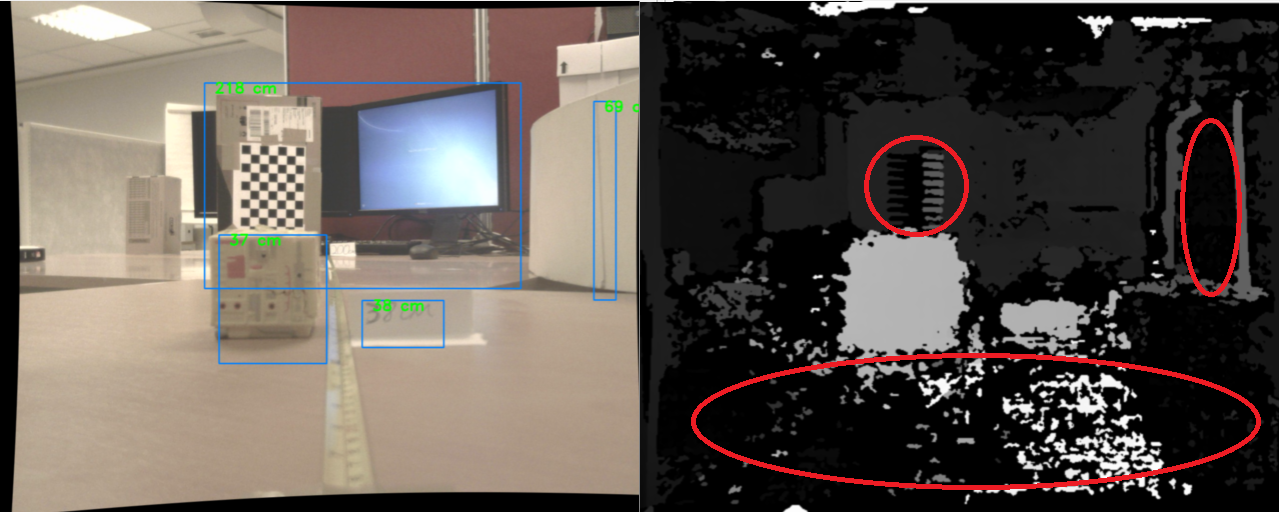
\includegraphics[width=\textwidth]{stereoWeakness}
	\caption{Illustration of the weaknesses with stereo matching. Little or no matching where there are few distinct features. False matches and shadows caused by repetitive patterns.}
	\label{fig:stereoWeakness}
\end{figure}



\subsection{Obstacle Detection}

Obstacle detection based on depth layers works as intended, and could potentially be adapted and improved for an obstacle avoidance system. Figure \ref{fig:contourDetection} in chapter \ref{chp:implementation} shows that several contours are placed closed to each other, thus resulting in an image cluttered with detected obstructions. While a cluttered image is not user friendly, it is not necessarily a problem in terms of obstacle detection. Note that this is an obstacle detector, not an object detector. This implies that it is sufficient to know that something is obstructing the path of the robot. 

\subsection{Hardware}

\paragraph{Cameras}

The two IP cameras proved to be up for the task of demonstrating basic real-time stereo matching, but not much more. Some of the disparity maps were surprisingly dense, but never as dense as the sample images used in the preliminary parts of the project (see figure \ref{fig:StereoGui}). When the rectified images are placed next to each other (figure \ref{fig:stereoPostCal), it looks like the imaging chips within the camera are misaligned. In addition, the stereo images were so dissimilar in color and brightness in the beginning of the project that matching was impossible, even when the camera settings were equal and calibrated. 


\subsection{Suitability for Autonomous Navigation}

The obstacle detector shows promise as a functionality in an autonomous system. However, the quality of the stereo map is currently too poor and prone too errors. Ground plane removal should also be solved, so that a clear path between two obstruction can be found. 